% !TEX root = sum1.tex
\section{Computational Experiments}\label{sec_result}
We carried out several experiments, including analyzing the performances of different policies, evaluating the impact of implementing social distancing, comparing different layouts, $M$s and social distancings. In the experiments, we set the following parameters. 

The default setting in the experiments is as follows, $\delta =1$ and $M =4$. The number of scenarios in SBSP is $|\Omega| = 1000$. The default seat layout consists of 10 rows, each with the same size of 21. Different realistic layouts, group sizes and social distances are also explored. We simulate the arrival of exactly one group in each period, i.e., $p_0 = 0$. The average number of individuals per period, denoted as $\gamma$, can be expressed as $\gamma = \sum_{i=1}^{M} i p_i$. Each experiment result is the average of 100 instances.
% The occupancy rate at different demands is calculated as the average of these 100 instances. 
% Each entry in the table represents the average performance across 100 instances.

\subsection{Performances of Different Policies}
In this section, we compare the performance of four assignment policies against the optimal one, which is derived by solving the deterministic model after observing all arrivals. The policies under evaluation are DSA, DP-based heuristic (DPBH), bid-price control (BPC), booking-limit control (BLC) policies.

\subsection*{Parameters Description}
We consider four probability distributions for our analysis. The first two, $D1:[0.18,0.7,0.06,0.06]$ and $D2:[0.2,0.8,0,0]$, were experimented with in \cite{blom2022filling}. Here, $D1$ represents the statistical distribution of group sizes, while $D2$ can be interpreted as a restricted situation where groups of more than 2 people are not allowed in our context. For additional experiments, we introduce two more distributions, $D3$ and $D4$, derived from real-world movie data.

Specifically, we selected Detective Chinatown 1900 and Captain America: Brave New World as target movies to analyze group information and their corresponding probability distributions, denoted as D3 and D4, respectively. The seat plans for the tickets were obtained from the MCL cinema website. We focused on scattered seat plans and excluded cases where the number of consecutive seats exceeded four. By counting the occurrences of different group types, we obtained the following distributions: $D3 = [0.34, 0.51, 0.07, 0.08]$ representing the suspense genre, and $D4: [0.12, 0.5, 0.13, 0.25]$, representing the family fun genre. To assess the effectiveness of different policies across varying demand levels, we conducted experiments spanning a range of 60 to 100 periods. 


The following table presents the performance results of four different policies: DSA, DPBH, BPC, BLC, which stand for dynamic seat assignment, dynamic programming-based heuristic, bid-price control and booking-limit control policies, respectively. The procedures of the BPC and BLC policies are detailed in Appendix \ref{policies}. Performance is evaluated by comparing the ratio of the number of accepted individuals under each policy to that under the optimal policy, which assumes complete knowledge of all incoming groups before making seat assignments.

\begin{table}[h]
  \centering
  \caption{Performances of Different Policies}
  \begin{tabular}{cc|cccc}
  \hline
  Distribution & T & DSA (\%) & DPBH (\%) & BPC (\%) & BLC (\%) \\
  % \Xcline{1-1}{0.4pt}\Xcline{3-3}{0.4pt}\Xcline{4-4}{0.4pt}
  % \cmidrule(r){0-1} \cmidrule(lr){3-3} \cmidrule(lr){4-4} \cmidrule(lr){5-5} \cmidrule(lr){6-6} \cmidrule(l){7-7}
  \hline
  \multirow{5}{*}{D1} & 60 & 100.00 & 100.00 & 100.00 & 88.56 \\
  & 70    & 99.53 & 99.01 & 98.98 & 92.69  \\
  & 80    & 99.38 & 98.91 & 98.84 & 97.06  \\
  & 90    & 99.52 & 99.23 & 99.10 & 98.24  \\
  & 100   & 99.58 & 99.27 & 98.95 & 98.46 \\
  \hline
  \multirow{5}{*}{D2} & 60  & 100.00 & 100.00 & 100.00 & 93.68  \\
     & 70  & 100.00 & 100.00 & 100.00 & 92.88  \\
     & 80  & 99.54 & 97.89 & 97.21 & 98.98  \\
     & 90  & 99.90 & 99.73 & 99.44 & 99.61  \\
     & 100 & 100.00 & 100.00 & 100.00 & 99.89  \\ 
  \hline
  \multirow{5}{*}{D3} & 60  & 100.00 & 100.00 & 100.00 & 91.07  \\
  & 70  & 99.85 & 99.76 & 99.73 & 90.15 \\
  & 80  & 99.22 & 98.92 & 98.40 & 96.98  \\
  & 90  & 99.39 & 99.12 & 98.36 & 96.93  \\
  & 100  & 99.32 & 99.18 & 98.88 & 97.63  \\
    \hline
    \multirow{5}{*}{D4} & 60  & 99.25 & 99.18 & 99.13 & 93.45  \\
     & 70  & 99.20 & 98.65 & 98.54 & 97.79  \\
     & 80  & 99.25 & 98.69 & 98.40 & 98.22 \\
     & 90  & 99.29 & 98.65 & 98.02 & 98.42  \\
     & 100 & 99.60 & 99.14 & 98.32 & 98.68 \\
  \hline
  \end{tabular}
\end{table}

We can find that DSA is better than DPBH, BPC and BLC policies consistently. DPBH and BPC policies can only decide to accept or deny, cannot decide which row to assign the group to. BLC policy does not consider using more seats to meet the demand of one group.

The performance of DSA, DP-based heuristic, and bid-price policies follows a pattern where it initially decreases and then gradually improves as $T$ increases. When $T$ is small, the demand for capacity is generally low, allowing these policies to achieve relatively optimal performance. However, as $T$ increases, it becomes more challenging for these policies to consistently achieve a perfect allocation plan, resulting in a decrease in performance. Nevertheless, as $T$ continues to grow, these policies tend to accept larger groups, thereby narrowing the gap between their performance and the optimal value. Consequently, their performances improve. In contrast, the booking-limit policy shows improved performance as $T$ increases because it reduces the number of unoccupied seats reserved for the largest groups. 

The performance of the policies can vary with different probabilities. For the different probability distributions listed, DSA performs more stably and consistently for the same demand. In contrast, the performance of DPBH and BPC fluctuates more significantly.


\subsection{Impact of Social Distancing}\label{impact_sd}
We examine the impact of social distancing when implementing DSA under varying levels of demand. As an illustrative example, we use $D4$ as the probability distribution. Two situations: $\delta =0$ (no social distancing) and $\delta = 1$ (with social distancing) are tested. The demand levels are varied by adjusting the parameter $T$ from 40 to 100 in increments of 1. 
The results are visualized in Figure \ref{occupancy_rate_demand}, which shows the occupancy rate under different demand levels. 

Additionally, Figure \ref{x_period} and \ref{x_demand} illustrate 

Figure \ref{x_period} displays Percentage of accepted individuals relative to total seats over period. Figure \ref{x_demand} displays Percentage of accepted individuals relative to total seats over demand. 



% It is evident that as the demand increases, the effect of social distancing becomes more pronounced. We aim to determine the specific time period where the absence of social distancing results in a higher number of accepted individuals compared to when social distancing measures are in place. Additionally, we will calculate the corresponding occupancy rate during this period.

% By analyzing and comparing the data, we can gain insights into the relation between demand, social distancing, the number of accepted individuals, and occupancy rates. This information is valuable for understanding the impact of social distancing policies on overall capacity utilization and making informed decisions regarding resource allocation and operational strategies.

% The figure below displays the number of assigned individuals over demand under two different conditions: with social distancing measure ($\delta =1$) and without social distancing measure ($\delta =0$). The figures depicting the results are presented below. The difference between these two figures is the x-axis, the left one is period, while the right one is the percentage of expected demand relative to total seats.


The gap point $\tilde{T}$ is defined as the largest value of $T$ for which the inequality $E(T; \delta =1)+1 \geq E(T; \delta = 0)$ holds, where $E(T; \delta =1)$ denotes the average number of accepted individuals by DSA with one seat as social distancing, $E(T; \delta = 0)$ denotes the average number of accepted individuals by DSA when there is no social distancing.

The occupancy rate corresponding to the gap point is referred to as the threshold occupancy rate. This rate represents the maximum demand that can be satisfied when the difference in the number of accepted individuals remains unaffected by social distancing constraints.

\begin{figure}[h]
  \centering
  \subfigure[]{
    \label{x_period}
    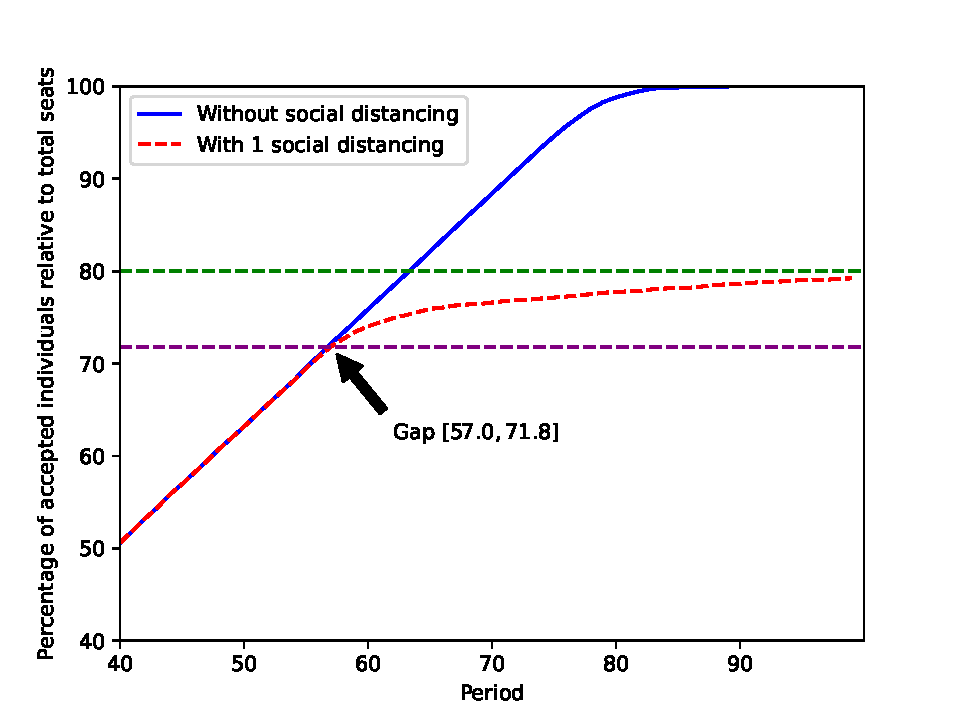
\includegraphics[width=0.48\textwidth]{./Figures/occu_demand.pdf}}
  \subfigure[]{
    \label{x_demand}
    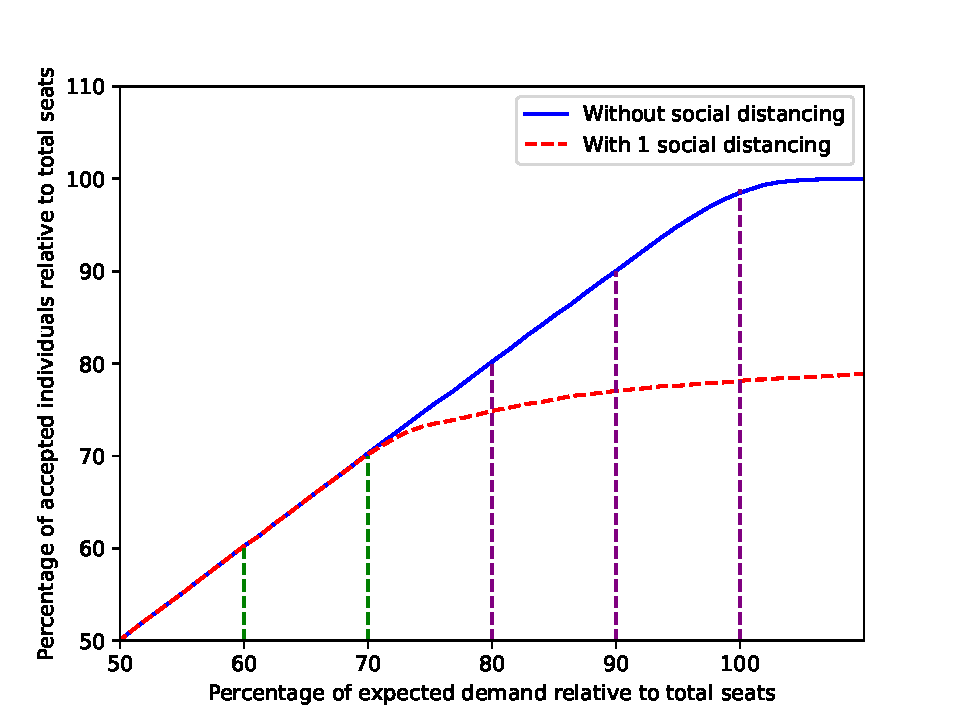
\includegraphics[width=0.48\textwidth]{./Figures/occu_gamma_group4.pdf}}
  \caption{The occupancy rate over demand}
  \label{occupancy_rate_demand}
\end{figure}

In figure \ref{x_period}, the gap point is 57, the threshold occupancy rate is 71.8\%. As the expected demand continues to increase, both situations reach their maximum capacity acceptance. For the social distancing situation, when the largest pattern is realized in each row, the maximum achievable occupancy rate is given by $\frac{16}{20} = 80\%$. The figure \ref{x_demand} is plotted to show that when the expected demand is less than 71.8\%, the social distancing measures will not have an impact; when the expected demand is larger than 71.8\%, the difference between the number of accepted individuals with and without social distancing measures becomes more pronounced.

\subsection*{Impact of Maximum Allowable Occupancy Rate}
Sometimes, policies impose a maximum allowable occupancy rate to enforce stricter social distancing. This maximum allowable rate becomes redundant if it exceeds the maximum achievable rate for all events. As shown by the green line in figure \ref{x_period}, when the maximum allowable rate is above 80\%, it has no effect. Only the occupancy rate requirement is effective, while the social distancing requirement becomes irrelevant for events with an occupancy rate below the threshold. This is illustrated by the purple line in figure \ref{x_period}, where a maximum allowable rate below 71.8\% renders only the occupancy rate requirement effective. Additionally, when the maximum allowable rate falls between the threshold occupancy rate and the maximum achievable rate, both the occupancy rate and social distancing requirements jointly influence seat assignments.

% Similarly, $\phi(M, L)$ does not decrease in $L$. Since any largest pattern $\bm{h}$ under $L$ is a feasible pattern under $L+1$, thus, $\phi(M, L) \leq \phi(M, L+1)$.

% \begin{figure}[ht]
%   \centering
%     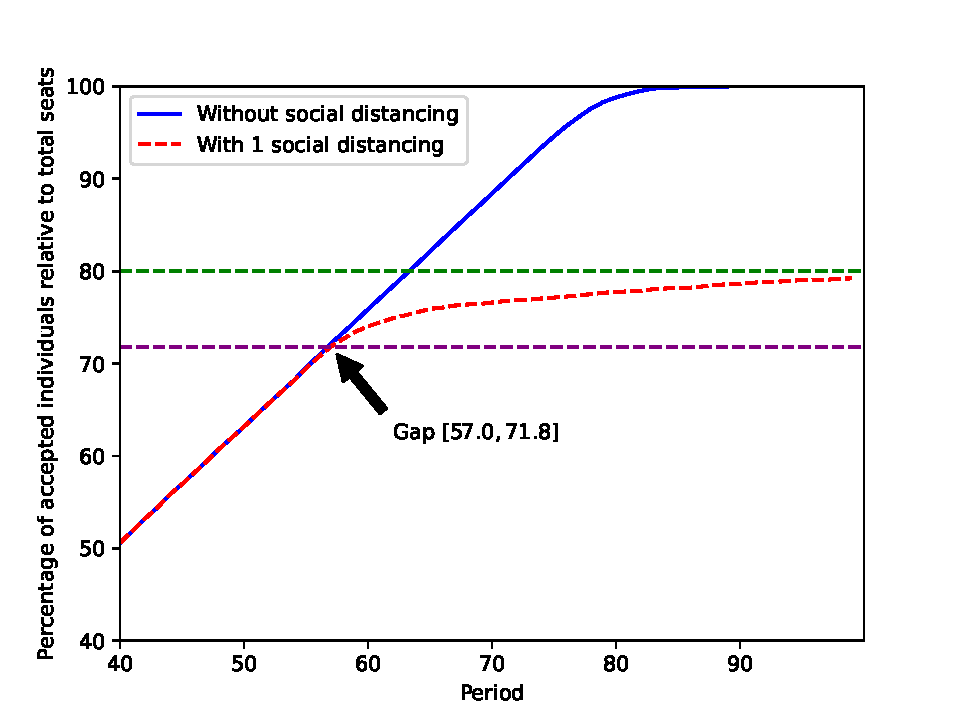
\includegraphics[width=0.95\textwidth]{./Figures/occu_demand.pdf}
%   \caption{The occupancy rate over demand}
% \end{figure}

% The policy requires a maximum allowable occupancy rate larger than 80\% will be redundant.

\subsection{Estimation of Gap Points}
To estimate the gap point, we aim to find the maximal period such that all requests can be assigned into the seats during these periods, i.e., for each group type $i$, we have $\bm{X}_{i} = \sum_{j} x_{ij} \geq d_i$. Meanwhile, we have the capacity constraint $\sum_{i} n_{i} x_{ij} \leq L_j$, thus, $\sum_{i} n_i d_i \leq \sum_{i} n_i \sum_{j} x_{ij} \leq \sum_{j} L_{j}$. Notice that $E(d_i) = p_i T$, we have $\sum_{i} n_i p_i T \leq \sum_{j} L_{j}$ by taking the expectation. Recall that $\tilde{L} = \sum_{j} L_{j}$ denotes the total number of seats, and $\gamma$ represents the average number of individuals in each period. Then, we can derive the inequality $T \leq \frac{\tilde{L}}{\gamma + \delta}$. Therefore, the upper bound for the expected maximal period is given by $T' = \frac{\tilde{L}}{\gamma + \delta}$.


Assuming that all arrivals within $T'$ periods are accepted and fill all the available seats, the threshold occupancy rate can be calculated as $\frac{\gamma T'}{(\gamma+ \delta)T' - N \delta} = \frac{\gamma}{\gamma +\delta} \frac{\tilde{L}}{\tilde{L}-N \delta}$. However, it is important to note that the actual maximal period will be smaller than $T{'}$ because it is nearly impossible to accept groups to fill all seats exactly. To estimate the gap point when applying DSA, we can use $y_1 = c_1 \frac{\tilde{L}}{\gamma + \delta}$, where $c_1$ is a discount factor compared to the ideal assumption. Similarly, we can estimate the threshold occupancy rate as $y_2 = c_2 \frac{\gamma}{\gamma +\delta} \frac{\tilde{L}}{\tilde{L}-N \delta}$, where $c_2$ is a discount factor for the occupancy rate compared to the ideal scenario.

To analyze the relation between $\gamma$ and the gap point, we conducted an analysis using a sample of 200 probability distributions. The figure below illustrates the gap point as a function of $\gamma$, along with the corresponding estimations.  Additionally, the threshold occupancy rate is represented by red points. 

We applied an Ordinary Least Squares (OLS) model to fit the data and estimate the parameter values. The resulting fitted equations, $y_1 = \frac{c_1 \tilde{L}}{\gamma + \delta}$ (represented by the blue line in the figure) and $y_2 = c_2 \frac{\gamma}{\gamma + \delta} \frac{\tilde{L}}{\tilde{L}-N \delta}$ (represented by the orange line in the figure), are displayed in the figure. The goodness of fit is evaluated using R-squared values, which are 1.000 for both models, indicating a perfect fit between the data and the fitted equations. The estimated discount factor values are $c_1 = 0.9578$ and $c_2 = 0.9576$.

\begin{figure}[ht]
  \centering
    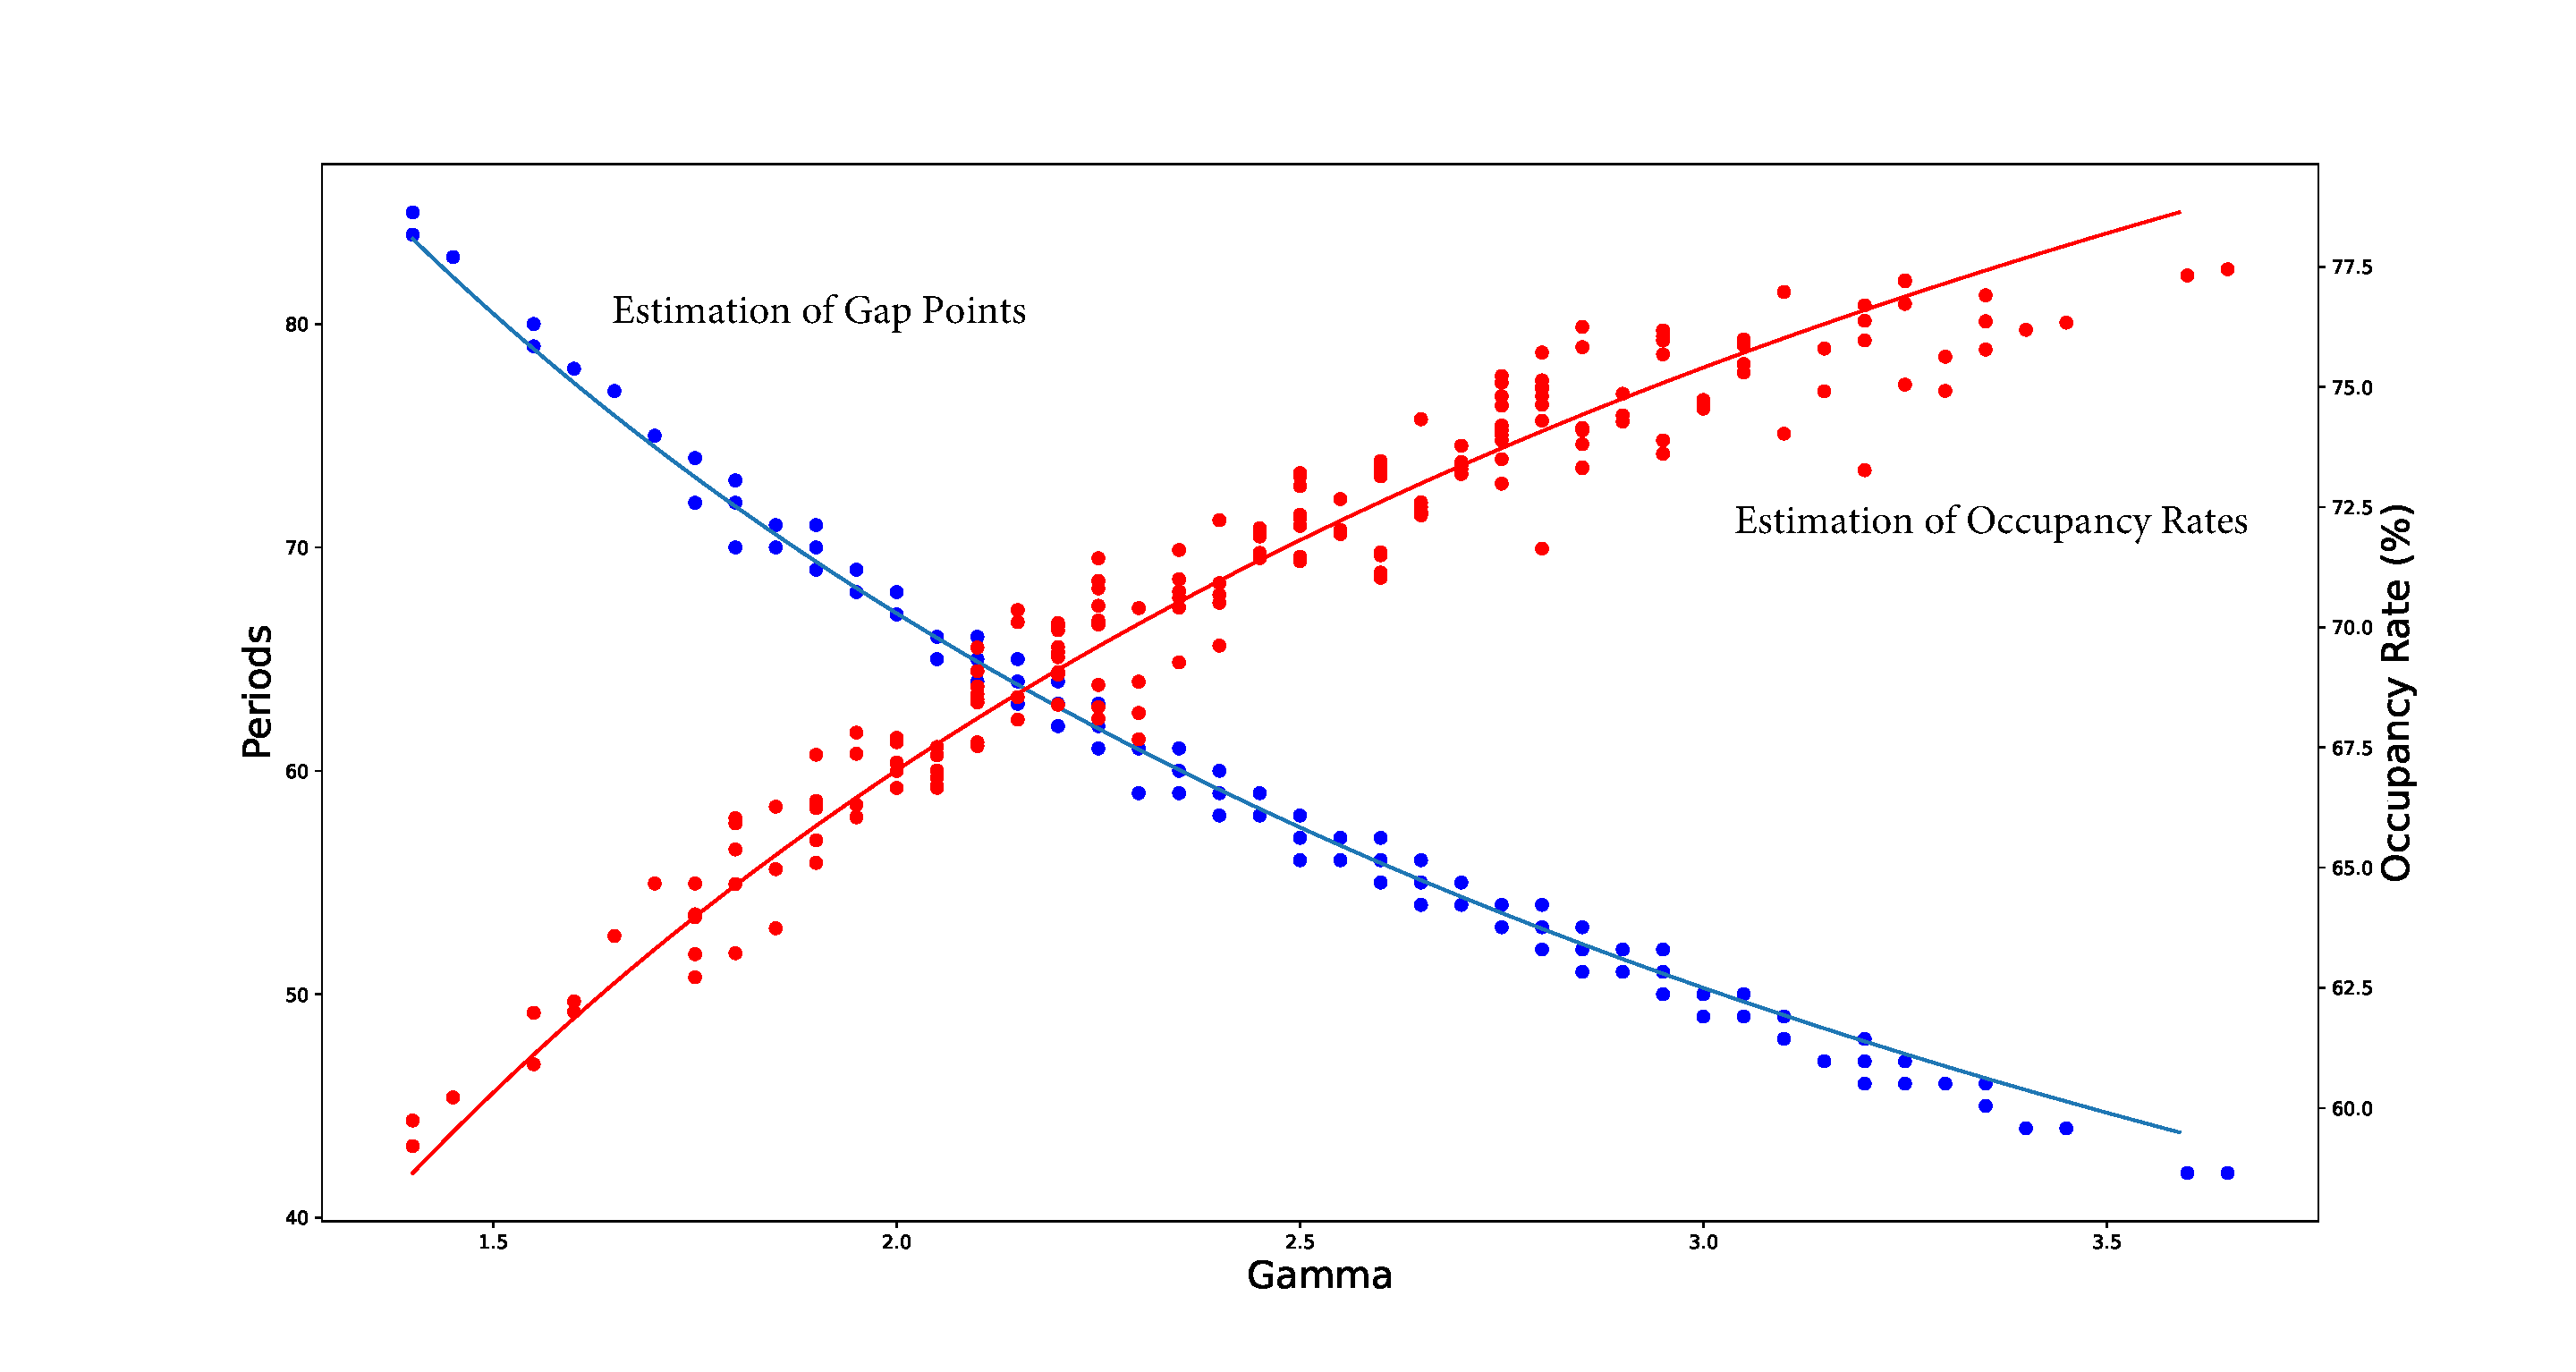
\includegraphics[width=0.95\textwidth]{./Figures/esti_scatter.pdf}
  \caption{Gap points and their estimation under 200 probabilities}
\end{figure}

% As the value of $\gamma$ increases, the gap point will decrease and the corresponding occupancy rate will increase. Consequently, the occupancy rate increases due to the allocation of seats to larger groups. The percentage difference is negligible when the demand is small, but it becomes more significant as the demand increases.

Based on the above analysis, we also explore the results of different layouts, different group sizes and different social distances. Since the figure about the occupancy rate over demand is similar to Figure \ref{occupancy_rate_demand}, we only use three metrics to show the results: the gap point and the threshold occupancy rate, maximal achievable occupancy rate.

\subsection*{Different Layouts}
We experiment with several realistic seat layouts selected from the theater seat plan website, https://www.lcsd.gov.hk/en/ticket/seat.html. We select five places, Hong Kong Film Archive Cinema, Kwai Tsing Theatre Transverse Stage, Sai Wan Ho Civic Centre, Sheung Wan Civic Centre, Ngau Chi Wan Civic Centre, represented as HKFAC, KTTTS, SWHCC, SWCC, NCWCC respectively. HKFAC, SWCC, NCWCC, are approximately rectangular layouts, SWHCC is a standard rectangular layout. While KTTTS is an irregular layout. In these layouts, wheelchair seats and management seats are excluded, while seats with sufficient space for an aisle are treated as new rows. 

The occupancy rate over demand follows the typical pattern of Figure \ref{occupancy_rate_demand}. The gap point, the threshold occupancy rate and the maximum achievable occupancy rate are also given in the following table. The maximum achievable occupancy rate can be calculated from Proposition \ref{lem_pattern}.

\begin{table}[ht]
  \centering
  \caption{Gap points and threshold occupancy rates of the layouts}
  \begin{tabular}{c|ccc}
  \hline
   Seat Layout & Gap point & Threshold occupancy rate & Maximum achievable occupancy rate \\
  %  \cmidrule(r){1-1} \cmidrule(lr){2-2} \cmidrule(lr){3-3} \cmidrule(l){4-4}
  \hline
   HKFAC & 36 & 72.3 \% & 82.4 \% \\
   KTTTS & 38 & 75.79 \% & 84.1 \% \\
   SWHCC & 32 & 72.83 \% & 80 \% \\
   SWCC & 43 & 74.07 \%  & 83.6 \% \\
   NCWCC & 102 & 72.37 \% & 81.7 \% \\
   \hline
  \end{tabular}
\end{table}

Generally speaking, the length of each row impacts the occupancy rate, as a full pattern can maximize seat utilization, leading to a higher occupancy rate. However, in rectangular layouts, achieving a full pattern in each row can be challenging, resulting in a relatively low occupancy rate, as seen in SWHCC. Although these layouts are all approximately rectangular, the varying lengths of each row lead to different occupancy rates, as demonstrated by HKFAC, SWCC, and NCWCC.

% This suggests that, when the total number of seats is the same, the layout with more rows yields a larger gap point and occupancy rate compared to the layout with fewer rows.

% For each row, a seat is designated for social distancing with every group accepted. Consequently, when each row follows a full pattern and the total number of seats remains constant, having more rows results in a higher gap point and occupancy rate. Similarly, in a small room with fewer seats per row, the occupancy rate at the gap point will correspondingly be higher.

\subsection*{Different Allowable Largest Group Sizes}
When $M$ is restricted at 3, given the probability distribution [0.12, 0.5, 0.13, 0.25], we discard the fourth component and normalize the remaining three components to generate a new probability distribution [0.16, 0.67, 0.17]. Similarly, when $M =2$, the probability distribution is [0.19, 0.81].
We present the gap point, the threshold occupancy rate and the maximum achievable occupancy rate in the table below.


\begin{table}[ht]
  \centering
  \caption{Gap points and threshold occupancy rates of $M$s}
  \begin{tabular}{c|ccc}
  \hline
   $M$  & Gap point & Threshold occupancy rate & Maximum achievable occupancy rate \\
  %  \cmidrule(r){1-1} \cmidrule(lr){2-2} \cmidrule(lr){3-3} \cmidrule(l){4-4}
  \hline
   2 &  74  & 66.88 \% & 70 \% \\
   3 &  69  & 69.03 \% & 75 \% \\
   4 &  57  & 71.82 \% & 80 \% \\ 
   \hline
  \end{tabular}
\end{table}

% We observe that larger group sizes correspond to higher largest occupancy rates under the same seat layout. However, the gap point and occupancy rate for larger group sizes do not necessarily increase correspondingly. The explanation for this is that as larger groups are allowed to be accepted, seat allocation makes it difficult to achieve a full pattern for each row. Thus, there will be a decrease in both gap points and occupancy rates, i.e., the impact of social distancing will manifest at an earlier period.

% The insight is although allowing larger groups will increase the largest occupancy rate, the impact of social distancing will become evident at an earlier period. Specifically, if demand is low or if the managers wish to avoid rejecting a significant number of customers, they can set a smaller group size limit. Conversely, when demand is high, a larger group size limit can be set to accommodate more customers.

\subsection*{Different Social Distances}
The following figure illustrates the number of accepted individuals over time with social distancing set at 0, 1, and 2 seats, respectively.

\begin{figure}[h]
  \centering
    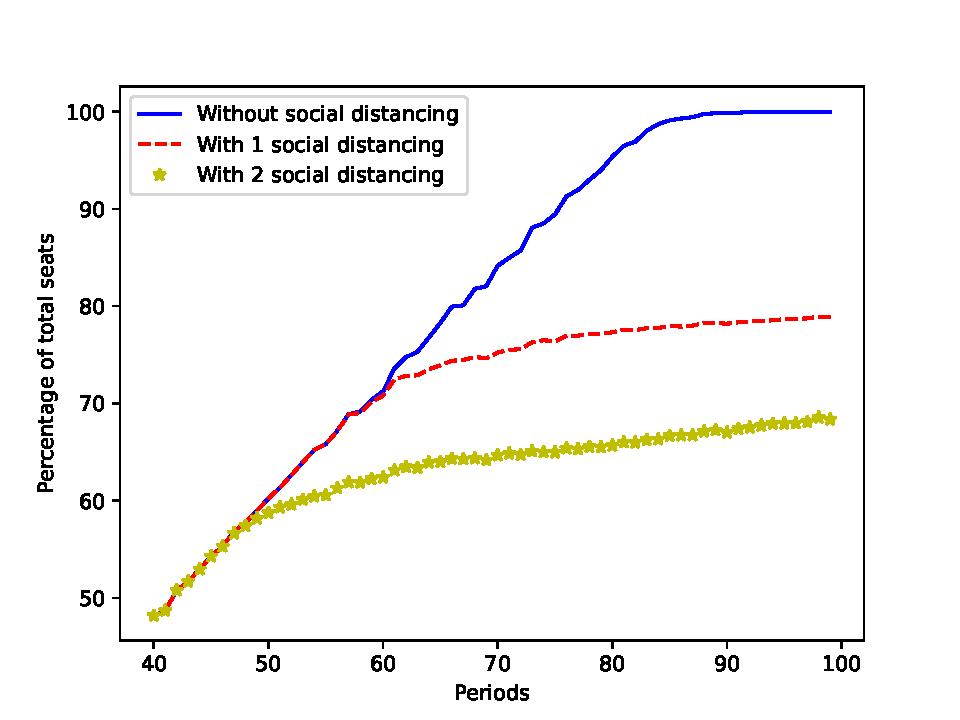
\includegraphics[width=0.8\textwidth]{./Figures/distance.pdf}
  \caption{The occupancy rate over demand for different social distancings}
\end{figure}

% We examine the impact of implementing social distancing on the occupancy rate and explore strategies to minimize revenue loss. Consider the situation where the gap point is $\tilde{T}$ and is determined by the parameters $\delta$, $\gamma$, $M$, and $\tilde{L}$. The corresponding occupancy rate is $\Gamma(\tilde{T})$. When the actual number of people (demand) is less than $\tilde{L} \cdot \Gamma(\tilde{T})$, implementing social distancing does not affect the revenue. However, if the actual number of people exceeds $\tilde{L} \cdot \Gamma(\tilde{T})$, enforcing social distancing measures will lead to a reduction in revenue. The extent of this loss can be assessed through simulations by using the specified parameters. To mitigate the potential loss, the seller can increase the value of $\gamma$. This can be achieved by implementing certain measures, such as setting a limit on the number of single-person groups or allowing for larger group sizes. 

% At times, the government may establish a maximum allowable occupancy rate. This rate is effective for an event only if it is lower than the expected occupancy rate. Additionally, the maximum allowed rate becomes redundant if it exceeds the maximum achievable rate for all events.

% for example, for family movies in cinemas, $\gamma$ will be relatively large, so a higher occupancy rate limit can be set.


% HONG KONG FILM ARCHIVE CINEMA [17, 18, 18, 18, 18, 18, 18, 8]

% Kwai Tsing Theatre Transverse Stage [7, 9, 7, 10, 7, 11, 8, 11, 9, 7, 10, 7, 11, 7, 13, 8]

%%  Kwai Tsing Theatre Arena Stage  [6, 6, 5, 7, 7, 7, 8, 8, 7, 7, 7, 7, 8, 8, 6, 4, 5, 5, 6, 6, 6, 6, 4, 6, 5, 5, 6, 6, 6, 6]

% Sai Wan Ho Civic Centre [6, 6, 6, 6, 6, 6, 6, 6, 6, 6, 6] 6* 22

% Sheung Wan Civic Centre [3, 13, 13, 13, 13, 13, 13, 13, 13, 13, 13, 13, 13]

% Ngau Chi Wan Civic Centre Theatre  [13, 21, 23, 23, 23, 23, 23, 23, 23, 23, 23, 23, 23, 23, 23, 21, 13]